\section{What fixes it}
\label{sec:fixes}

\Cref{sec:diagnosis} shows that matching the small views to the sharp ones recovers most of the loss for \pithree and \dathree. Upsampling does this at roughly twice the token cost ($\rho{=}2$) or 2.5 times ($\rho{=}3$), so it is a diagnostic rather than a fix. Here we ask what can be done at no extra cost, first inside the model and then at the input.

\subsection{Corrections inside the model help a little}

\paragraph{Position alignment.}
In a small view, patch $p$ on a grid of $g$ patches per axis sits at a different relative location than patch $p$ on the sharp grid of $g_{\mathrm{ref}}$ patches. We map each small-view position onto the sharp grid,
\begin{equation}
  \tilde p \;=\; \Big(p+\tfrac12\Big)\frac{g_{\mathrm{ref}}}{g} - \tfrac12 ,
  \label{eq:align}
\end{equation}
per axis, so that patch centres cover the same part of the image in both views. Among training-free position policies tested on the selection seed, this ties for best on \pithree: pooled over three datasets, it scores 3.02 \auc, the same as a frequency-split variant, against 3.00 for YaRN~\cite{peng2023yarn}, 2.88 for CRPA-style re-indexing~\cite{crpa2025} and 0.73 for native positions. The best policies differ by at most 0.14 \auc, and none lifts the pooled score above about 3; VGGT stays at its floor under every policy. On the reporting seed, alignment beats the as-is mix in 7 of 10 pose cells for \pithree and 5 of 10 for both \dathree and VGGT, without a loss (\cref{tab:diag}), but on HiRoom it moves \pithree only from 0.8 to 12.5 of the 60.9 that sharp input reaches.

\paragraph{Attention correction.}
A small view has fewer tokens than the model saw in training, which changes how spread out its frame attention is. Following Jin \etal~\cite{jin2023training}, we scale the frame-attention queries of a small view with $N$ patches by
\begin{equation}
  \lambda \;=\; \sqrt{\frac{\log N}{\log T}}\quad (N<T), \qquad \lambda=1 \quad (N\ge T),
  \label{eq:lambda}
\end{equation}
where $T$ is the model's default patch count (\cref{tab:models}). On top of alignment, it helps \pithree in 6 of 10 pose cells without a loss, helps \dathree in 2 and hurts it in 1, and barely changes reconstruction (\cref{tab:diag}). Studies on the selection seed show where its benefit comes from, and two of our predictions about it failed. Its benefit comes entirely from the small views: applied to them alone it gives \pithree a pooled 4.56 \auc, against 2.85 when applied to the sharp views alone. A version calibrated per layer and head to restore attention entropy, fitted on held-out data, kept almost none of the gain, so restoring entropy is not what makes it work. A correction strength chosen on held-out data hurt \pithree on 7-Scenes. Applied to the frozen mixes of \cref{sec:budget}, the correction helps in 4 of 24 pose cells and hurts in 9, mostly for \dathree. We therefore recommend it for \pithree only.

\subsection{Fixing the input works at the same cost}

\paragraph{One size for all views.}
Instead of upsampling, we resize all 12 views to the single resolution $r_{\mathrm{eq}}$ at which they cost exactly as many tokens as the mix. Sharp views lose some detail and small views gain size, but no view differs from another. This beats the aligned mix in 7 of 10 pose cells for \pithree and 4 of 10 for \dathree, with no losses. On HiRoom at $\rho{=}2$, \pithree rises from 12.5 to 42.3 \auc. Real pixels at that same size would give 44.6, and across datasets they add only $+1.4$ \auc for \pithree and $+0.8$ for \dathree on average, so the resized views lose little by being resampled. VGGT is the exception again, with 1 win and 4 losses: at the mix's cost each of its views gets only about 220 tokens, which is too few for it.

\paragraph{Equal detail at the same cost.}
Blurring all views to the small views' detail and then resizing them to one size within the mix's cost beats the aligned mix in 17 of 20 cells for \pithree and 18 of 20 for \dathree, again without losses. For VGGT it wins 3 and loses 5. We predicted that it would help VGGT at the higher token level; at $\rho{=}2$ that prediction held in only 1 of 5 cells.

\paragraph{For pose, fewer views can be better.}
At the mix's cost, the four sharp views alone give better pose than all 12 views at one size in 23 of 30 cells (6 of 10 for \pithree, 8 of 10 for \dathree, 9 of 10 for VGGT), with none the other way; on the four common frames this holds in 20 of 30. \Cref{fig:views} asks how many views to keep. At about 470 tokens per sharp view, fewer views are better; at about 1{,}000, a few extra views help. Over both levels, six views at one size beat twelve in 5 of 20 cells for \pithree (losing 1), 10 of 20 for \dathree and 12 of 20 for VGGT (losing none). Against the four sharp views alone, however, six views mostly lose (W/L of 0/4, 1/5 and 2/11 for \pithree, \dathree and VGGT). The clearest gain is VGGT on DTU, where six views reach 94.9 \auc against 79.5 for four, scored on the common frames; over all pairs the six-view input scores 80.3. We read this as a rule of thumb, about six views at one size when the budget gives each view enough tokens, rather than a fixed optimum.

\paragraph{Shrinking every view.}
A cheaper alternative is to shrink the sharp views to the small size, so all 12 views match at a lower cost. Whether this rescues the mix depends on how large the small views are. At the higher token level, it beats the aligned mix in 7 of 10 cells for \pithree, with no losses; on HiRoom at $\rho{=}2$, 12 small views reach 50.1 \auc with 3{,}072 tokens, against 15.0 for the aligned mix with 6{,}144. At the lower level, where small views are about 175\,px, the result is split (3 wins, 3 losses), and for \dathree and VGGT it does not hold: for VGGT the mix wins all 10 cells at the higher level. Even where shrinking helps \pithree, it gives it more usable views at the price of worse sharp frames: scored on the common frames at the higher level, shrinking loses to the mix in 5 cells and wins in 2. Shrinking never beats the four sharp views alone (0 wins, 53 losses in 60 cells). It is not a general replacement for the other fixes.

\begin{figure}[t]
  \centering
  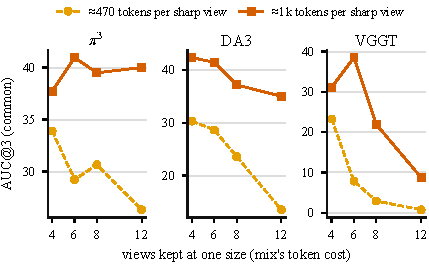
\includegraphics[width=\linewidth]{figures/fig_views.pdf}
  \caption{\textbf{How many views to keep at the mix's token cost.} Pose \auc on the 4 common sharp frames, mean over five datasets ($\rho{=}2$), when the 4 sharp views plus 0, 2, 4 or 8 small views are all resized to one size within the mix's cost. At about 470 tokens per sharp view, fewer views are better; at about 1{,}000, a few extra views help, most clearly for VGGT at 6 views.}
  \label{fig:views}
\end{figure}

\paragraph{Graded mixes.}
The same conclusions hold when the 8 small views come in four sizes. Resizing all views to one size at the mix's cost beats the aligned mix in 9 of 10 cells for \pithree and 7 of 10 for \dathree without a loss, and loses 8 of 10 for VGGT. Twelve views at one size never beat the four sharp views alone for \pithree (0 wins, 3 losses) or VGGT (0 wins, 9 losses), and rarely for \dathree (1 win, 5 losses). Grading the sizes does not create a regime in which mixing pays.

\paragraph{A recipe.}
\Cref{tab:recipe} turns these results into advice for inputs that arrive mixed. For \pithree and \dathree, the best option is to upsample the small views if the budget allows, and otherwise to resize every view to one size. For VGGT, pose is best with the small views left out: on ETH3D the four sharp views score 6.1 \auc against 5.9 for twelve sharp views, and on DTU 36.6 against 32.7. For VGGT reconstruction at $\rho{=}2$, the small views should be kept with aligned positions (F-score 0.166 against 0.113 without them, ETH3D), and at $\rho{=}3$ dropped (0.057 against 0.113).

\begin{table}[t]
\centering\small
\setlength{\tabcolsep}{3pt}
\begin{tabular}{@{}lll@{}}
\toprule
Model & Pose & Reconstruction \\
\midrule
\pithree & Upsample (+ attention) & Upsample \\
\dathree & Upsample & Upsample \\
VGGT     & Drop small views & $\rho{=}2$: keep, aligned; $\rho{\ge}3$: drop \\
\midrule
\multicolumn{3}{@{}l@{}}{\emph{At the mix's token cost:} one size for all views (\pithree, \dathree);} \\
\multicolumn{3}{@{}l@{}}{\quad the sharp views only (VGGT, and pose at low tokens per view).} \\
\bottomrule
\end{tabular}
\caption{\textbf{What to do with an input that arrives mixed.} Derived from the reporting-seed results of \cref{sec:diagnosis,sec:fixes}.}
\label{tab:recipe}
\end{table}
